\documentclass[12pt, a4paper]{report}

%% ─── Packages ────────────────────────────────────────────────────────────────
\usepackage[a4paper, top=25mm, bottom=25mm, left=25mm, right=22mm]{geometry}
\usepackage[utf8]{inputenc}
\usepackage[T1]{fontenc}
\usepackage{lmodern}
\usepackage{microtype}
\usepackage{amsmath, amssymb, bm}
\usepackage{booktabs}
\usepackage{array}
\usepackage{longtable}
\usepackage{tabularx}
\usepackage{multirow}
\usepackage{colortbl}
\usepackage[dvipsnames,svgnames,x11names]{xcolor}
\usepackage{graphicx}
\usepackage{tikz}
\usepackage{pgfplots}
\pgfplotsset{compat=1.18}
\usetikzlibrary{shapes,arrows.meta,positioning,calc,fit,backgrounds,decorations.pathreplacing}
\usepackage{tcolorbox}
\tcbuselibrary{skins, breakable, theorems}
\usepackage{enumitem}
\usepackage{fancyhdr}
\usepackage{titlesec}
\usepackage{titletoc}
\usepackage[hidelinks]{hyperref}
\usepackage{cleveref}
\usepackage{parskip}
\usepackage{setspace}
\usepackage{caption}
\usepackage{subcaption}
\usepackage{pifont}
\usepackage{fontawesome5}
\usepackage{mdframed}
\usepackage{listings}
\usepackage{mathtools}

%% ─── Colours ─────────────────────────────────────────────────────────────────
\definecolor{sambpblue}{RGB}{31, 78, 121}
\definecolor{sambpred}{RGB}{180, 40, 40}
\definecolor{sambpgreen}{RGB}{0, 112, 60}
\definecolor{sambporange}{RGB}{200, 100, 0}
\definecolor{sambppurple}{RGB}{90, 40, 130}
\definecolor{sambpgray}{RGB}{80, 80, 90}
\definecolor{lightblue}{RGB}{220, 235, 252}
\definecolor{lightgreen}{RGB}{220, 245, 230}
\definecolor{lightyellow}{RGB}{255, 252, 220}
\definecolor{lightorange}{RGB}{255, 240, 220}
\definecolor{lightpurple}{RGB}{240, 230, 255}
\definecolor{lightred}{RGB}{255, 230, 230}
\definecolor{darkgray}{RGB}{50,50,60}

%% ─── Page style ──────────────────────────────────────────────────────────────
\pagestyle{fancy}
\fancyhf{}
\fancyhead[L]{\small\textcolor{sambpgray}{\leftmark}}
\fancyhead[R]{\small\textcolor{sambpgray}{SAMBP Research Gap-Filling Plan}}
\fancyfoot[C]{\small\textcolor{sambpgray}{\thepage}}
\renewcommand{\headrulewidth}{0.4pt}
\renewcommand{\headrule}{\hbox to\headwidth{\color{sambpblue}\leaders\hrule height \headrulewidth\hfill}}

%% ─── Section formatting ──────────────────────────────────────────────────────
\newcommand{\chaptitlebox}[1]{%
  \colorbox{sambpblue}{\parbox{\dimexpr\textwidth-2\fboxsep\relax}{%
    \color{white}\Large\bfseries\strut\quad #1\strut}}}
\titleformat{\chapter}[display]
  {\normalfont}{}
  {0pt}{\chaptitlebox}[\vspace{2pt}]
\titlespacing{\chapter}{0pt}{0pt}{18pt}

\titleformat{\section}{\large\bfseries\color{sambpblue}}{}{0pt}{}[{\titlerule[0.5pt]}]
\titlespacing{\section}{0pt}{14pt}{6pt}

\titleformat{\subsection}{\normalsize\bfseries\color{sambpgray}}{}{0pt}{}
\titlespacing{\subsection}{0pt}{10pt}{4pt}

\titleformat{\subsubsection}{\normalsize\itshape\color{sambpgray}}{}{0pt}{}
\titlespacing{\subsubsection}{0pt}{8pt}{3pt}

%% ─── tcolorbox styles ────────────────────────────────────────────────────────
\tcbset{
  gapbox/.style={
    enhanced, breakable,
    colback=lightblue, colframe=sambpblue,
    boxrule=0.8pt, arc=4pt,
    fonttitle=\bfseries\small\color{white},
    attach boxed title to top left={yshift=-2mm, xshift=6mm},
    boxed title style={colback=sambpblue, arc=3pt, boxrule=0pt},
    left=6pt, right=6pt, top=8pt, bottom=6pt,
  },
  mathbox/.style={
    enhanced, breakable,
    colback=gray!5, colframe=sambpgray,
    boxrule=0.5pt, arc=3pt,
    left=8pt, right=8pt, top=6pt, bottom=6pt,
    fontupper=\small,
  },
  ipbox/.style={
    enhanced, breakable,
    colback=lightyellow, colframe=sambporange,
    boxrule=0.8pt, arc=4pt,
    fonttitle=\bfseries\small\color{white},
    attach boxed title to top left={yshift=-2mm, xshift=6mm},
    boxed title style={colback=sambporange, arc=3pt, boxrule=0pt},
    left=6pt, right=6pt, top=8pt, bottom=6pt,
  },
  pubbox/.style={
    enhanced, breakable,
    colback=lightgreen, colframe=sambpgreen,
    boxrule=0.8pt, arc=4pt,
    fonttitle=\bfseries\small\color{white},
    attach boxed title to top left={yshift=-2mm, xshift=6mm},
    boxed title style={colback=sambpgreen, arc=3pt, boxrule=0pt},
    left=6pt, right=6pt, top=8pt, bottom=6pt,
  },
  noveltystar/.style={
    enhanced,
    colback=lightyellow, colframe=sambporange!60,
    boxrule=0.4pt, arc=2pt,
    left=3pt, right=3pt, top=2pt, bottom=2pt,
    fontupper=\small,
  },
  notebox/.style={
    enhanced, breakable,
    colback=lightpurple, colframe=sambppurple,
    boxrule=0.6pt, arc=4pt,
    left=6pt, right=6pt, top=6pt, bottom=6pt,
    fontupper=\small,
  },
}

%% ─── Custom commands ─────────────────────────────────────────────────────────
\newcommand{\trbox}[1]{\colorbox{sambpblue}{\textcolor{white}{\textbf{\small #1}}}}
\newcommand{\novelty}[1]{%
  \foreach \i in {1,...,5}{%
    \ifnum\i>#1\relax\textcolor{gray!40}{\ding{72}}\else\textcolor{sambporange}{\ding{72}}\fi%
  }%
}
\newcommand{\gap}[1]{\textcolor{sambpred}{\textbf{Gap:}} #1}
\newcommand{\eqnref}[1]{Eq.~(\ref{#1})}
\newcommand{\vect}[1]{\boldsymbol{#1}}
\newcommand{\mat}[1]{\mathbf{#1}}
\newcommand{\norm}[1]{\left\lVert#1\right\rVert}
\newcommand{\jj}{j\mkern1mu}

% Novelty bar command
\newcommand{\noveltybar}[1]{%
  \begin{tikzpicture}[baseline=-0.5ex]
    \foreach \i in {1,...,5}{
      \pgfmathparse{\i <= #1 ? 1 : 0}
      \ifnum\pgfmathresult=1
        \fill[sambporange] ({(\i-1)*0.22},0) rectangle ++(0.18,0.14);
      \else
        \fill[gray!25] ({(\i-1)*0.22},0) rectangle ++(0.18,0.14);
      \fi
    }
  \end{tikzpicture}%
}

%% ─── Table column types ──────────────────────────────────────────────────────
\newcolumntype{L}[1]{>{\raggedright\arraybackslash}p{#1}}
\newcolumntype{C}[1]{>{\centering\arraybackslash}p{#1}}

%% ─── Listing style (for pseudocode) ─────────────────────────────────────────
\lstset{
  basicstyle=\ttfamily\footnotesize,
  backgroundcolor=\color{gray!8},
  frame=single, framerule=0.3pt, rulecolor=\color{gray!50},
  breaklines=true, columns=flexible,
  xleftmargin=8pt, xrightmargin=4pt,
}

%% ═════════════════════════════════════════════════════════════════════════════
\begin{document}
%% ═════════════════════════════════════════════════════════════════════════════

%% ─── Title page ──────────────────────────────────────────────────────────────
\begin{titlepage}
\pagecolor{sambpblue}
\color{white}
\vspace*{1cm}
\begin{center}
  {\fontsize{11}{14}\selectfont\textbf{IIT MADRAS — PhD THESIS RESEARCH}}\\[6pt]
  {\fontsize{11}{14}\selectfont SAMBP: Smart Adaptive Model-Based Protection}\\[30pt]
  \rule{\textwidth}{1pt}\\[12pt]
  {\fontsize{24}{30}\selectfont\bfseries Research Gap-Filling Plan}\\[8pt]
  {\fontsize{18}{24}\selectfont\bfseries Novel Research Agenda}\\[8pt]
  {\fontsize{14}{18}\selectfont TR-56 through TR-67}\\[12pt]
  \rule{\textwidth}{1pt}\\[30pt]

  \begin{tikzpicture}
    \node[draw=white, fill=white!10, rounded corners=8pt,
          text width=14cm, align=center, inner sep=14pt] {
      \color{white}
      \textbf{Five Unresolved Gaps Addressed:}\\[8pt]
      \small
      G1: DFIG / Wind Generator Fault Modelling \quad
      G2: Solar PV Protection\\[4pt]
      G3: Transformer 87T IBR Extensions \quad
      G4: Generator Differential 87G\\[4pt]
      G5: Generator Protection Suite (Relay 40, 78, 64G, 81)
    };
  \end{tikzpicture}

  \vfill
  {\large April 2026}\\[6pt]
  {\normalsize Prepared for: PhD Thesis and Publication Pipeline}\\[4pt]
  {\normalsize 12 Proposed Technical Reports $\cdot$ 9 Journal Papers $\cdot$ 6 Patents $\cdot$ 5 Conference Papers}
\end{center}
\end{titlepage}
\nopagecolor

%% ─── Table of contents ───────────────────────────────────────────────────────
\tableofcontents
\clearpage

%% ═════════════════════════════════════════════════════════════════════════════
\chapter{Executive Summary and Priority Ranking}
%% ═════════════════════════════════════════════════════════════════════════════

\section{Context and Starting Point}

The SAMBP (Smart Adaptive Model-Based Protection) project developed a unified inverse-estimation framework for power system protection across 53 technical reports (TR-03 to TR-55). The core innovation is fitting a physics-based parametric model to measured fault current waveforms using Levenberg--Marquardt (LM) optimisation, then gating trip decisions on estimation confidence metrics ($\kappa_n$, $f_\mathrm{int}$, $\gamma$).

\medskip
The existing SAMBP framework addressed:
\begin{itemize}[nosep]
  \item \textbf{87L} line differential (SG and IBR networks) — most comprehensive coverage (TR-03 to TR-27)
  \item \textbf{87B} busbar differential — full topology coverage including GOOSE reconfiguration
  \item \textbf{87T} transformer differential — foundational framework only (TR-04)
  \item \textbf{21} distance relay — SG Mho and IBR cross-polar / quadrilateral / POTT
  \item \textbf{67N/67Q} directional overcurrent — IBR-specific
  \item \textbf{Adaptive OC 50/51} — synchronous generators and IBR microgrids
\end{itemize}

\begin{tcolorbox}[notebox, title={}]
\textbf{The coverage gap:} All SAMBP protection was developed with either (a) a synchronous generator (SG) source or (b) a generic inverter-based resource (IBR) source. No work specifically addressed DFIG wind generators, solar PV inverters, transformer protection under IBR, generator protection relay elements (40, 78, 64G, 81), or the 87G generator differential for any generator type.
\end{tcolorbox}

\section{Prioritisation Principle}

Research items are ranked by \textit{mathematical novelty and disruption to existing protection standards}. An item scores highest if it:
\begin{enumerate}[nosep]
  \item Invalidates a current IEC/IEEE standard assumption in an IBR context
  \item Introduces a genuinely new mathematical method to protection engineering
  \item Has high commercial IP potential (replaces relay hardware or changes relay settings)
\end{enumerate}

\section{Master Priority Table}

\begin{center}
\renewcommand{\arraystretch}{1.35}
\begin{tabular}{C{0.6cm} C{1.0cm} L{4.8cm} L{5.6cm} C{1.4cm}}
\toprule
\rowcolor{sambpblue}
\textcolor{white}{\textbf{\#}} &
\textcolor{white}{\textbf{TR}} &
\textcolor{white}{\textbf{Research Topic}} &
\textcolor{white}{\textbf{Core Mathematical Challenge}} &
\textcolor{white}{\textbf{Novelty}} \\
\midrule
1 & TR-56 & DFIG fault model + inverse estimation &
  Piecewise-ODE with unknown crowbar breakpoint; smoothed Heaviside LM &
  \noveltybar{5} \\
\rowcolor{lightblue}
2 & TR-57 & Bayesian SPRT for 87T inrush / fault &
  3-hypothesis sequential probability ratio test on waveform asymmetry &
  \noveltybar{5} \\
3 & TR-58 & Out-of-step (78) for hybrid SG--IBR &
  Generalised equal-area criterion; Lyapunov function for coupled ODEs &
  \noveltybar{5} \\
\rowcolor{lightblue}
4 & TR-59 & Virtual 87G-DFIG using EKF observer &
  Slip-frequency EKF rotor current estimation without rotor CTs &
  \noveltybar{4} \\
5 & TR-60 & Loss-of-excitation (40) with IBR &
  Nonlinear IBR admittance correction to classical Mho circles &
  \noveltybar{4} \\
\rowcolor{lightblue}
6 & TR-61 & Stator earth fault (64G) via injection &
  Optimal sub-harmonic injection frequency from SNR maximisation &
  \noveltybar{4} \\
7 & TR-62 & Solar PV sparse inverse model &
  2-parameter zero-DC model; k$_\mathrm{ibr}$-driven model selection &
  \noveltybar{3} \\
\rowcolor{lightblue}
8 & TR-63 & Under/over-frequency (81) zero-inertia &
  Inertia-normalised frequency deviation index for GFM networks &
  \noveltybar{3} \\
9 & TR-64 & 87T IBR system integration &
  SPRT + sparse model integration across all transformer topologies &
  \noveltybar{3} \\
\rowcolor{lightblue}
10 & TR-65 & Complete generator protection relay &
  Integration of TR-56--TR-63 into unified relay specification &
  \noveltybar{2} \\
11 & TR-66 & Monte Carlo robustness study &
  10{,}000-trial parametric validation of all new elements &
  \noveltybar{2} \\
\rowcolor{lightblue}
12 & TR-67 & HIL validation protocol extension &
  Hardware-in-the-loop with DFIG and PV emulators &
  \noveltybar{2} \\
\bottomrule
\end{tabular}
\end{center}

%% ═════════════════════════════════════════════════════════════════════════════
\chapter{Phase 1: Foundational Mathematics (Priority 1--3)}
%% ═════════════════════════════════════════════════════════════════════════════

\section{TR-56: Piecewise-ODE Fault Model for DFIG with Unknown Crowbar Breakpoint}

\begin{tcolorbox}[gapbox, title={Research Gap — TR-56}]
All existing SAMBP inverse-estimation models (TR-03, sync\_oc) assume a \textbf{continuously differentiable} fault current governed by a single ODE system. The DFIG Type-3 wind generator violates this assumption: when rotor current exceeds the crowbar threshold $I_\mathrm{cb}$, the crowbar fires and \textbf{discontinuously inserts} resistance $R_\mathrm{cb}$ into the rotor circuit. The fault current transitions at an \textit{a priori unknown} switching time $t_\mathrm{cb}$. \textbf{No existing protection inverse-estimation framework handles unknown breakpoints in piecewise-ODE systems.}
\end{tcolorbox}

\subsection{Mathematical Formulation}

\subsubsection{Pre-crowbar fault current ($t_0 \le t < t_\mathrm{cb}$)}

\begin{tcolorbox}[mathbox]
\begin{align}
  i_a(t) &= I_\mathrm{ss}\sin(\omega_s t + \phi_0)
           + I_\mathrm{nat}\sin\!\bigl((1-s)\omega_s t + \psi\bigr)\exp\!\left(-\frac{t-t_0}{\tau_r'}\right)
           + I_\mathrm{dc}\exp\!\left(-\frac{t-t_0}{\tau_s'}\right)\sin(\phi_0)
\end{align}
where $\tau_r' = L_r'/R_r \approx 0.5$--$2\,\mathrm{s}$ and $\tau_s' = L_s'/R_s \approx 20$--$200\,\mathrm{ms}$.
\end{tcolorbox}

\subsubsection{Post-crowbar model ($t \ge t_\mathrm{cb}$)}

\begin{tcolorbox}[mathbox]
\begin{align}
  i_a(t) &= I_\mathrm{ss}\sin(\omega_s t + \phi_\mathrm{cb})
           + I_\mathrm{nat}''\sin\!\bigl((1-s)\omega_s t + \psi_\mathrm{cb}\bigr)\exp\!\left(-\frac{t-t_\mathrm{cb}}{\tau_r''}\right)
           + I_\mathrm{dc}''\exp\!\left(-\frac{t-t_\mathrm{cb}}{\tau_s''}\right)\sin(\phi_\mathrm{cb})
\end{align}
where $\tau_r'' = L_r'/(R_r + R_\mathrm{cb}) \ll \tau_r'$ (crowbar collapses $\tau_r'$ from $\sim$1\,s to 5--30\,ms).
\end{tcolorbox}

\subsubsection{Full DFIG parameter vector}

\begin{equation}
  \vect{\theta}_\mathrm{DFIG} = \bigl[t_0,\ t_\mathrm{cb},\ I_\mathrm{ss},\ I_\mathrm{nat},\ \tau_r',\ \tau_s',\ I_\mathrm{nat}'',\ \tau_r'',\ \tau_s'',\ \phi_0\bigr]^\top \in \mathbb{R}^{10}
\end{equation}

\subsubsection{Novel mathematical problem: unknown breakpoint $t_\mathrm{cb}$}

The cost function $F(\vect{\theta}_\mathrm{DFIG}) = \norm{\vect{r}(\vect{\theta}_\mathrm{DFIG})}^2$ is \textbf{non-smooth} in $t_\mathrm{cb}$ because the model switches discretely. Standard LM cannot converge.

\textbf{Proposed solution — Smoothed Heaviside continuation:}

\begin{tcolorbox}[mathbox]
\begin{align}
  h_\varepsilon(t,\, t_\mathrm{cb}) &= \sigma\!\left(\frac{t - t_\mathrm{cb}}{\varepsilon}\right)
      = \frac{1}{1 + \exp(-(t-t_\mathrm{cb})/\varepsilon)} \label{eq:heaviside}\\[6pt]
  \hat{i}(t;\,\vect{\theta},\varepsilon) &= \bigl[1-h_\varepsilon\bigr]\cdot i_\mathrm{pre}(t;\,\vect{\theta}_\mathrm{pre})
                                          + h_\varepsilon \cdot i_\mathrm{post}(t;\,\vect{\theta}_\mathrm{post}) \label{eq:composite}\\[6pt]
  \frac{\partial \hat{i}}{\partial t_\mathrm{cb}} &= -\frac{1}{\varepsilon}\,h_\varepsilon(1-h_\varepsilon)\,
      \bigl[i_\mathrm{post} - i_\mathrm{pre}\bigr]
      \quad\longrightarrow\quad \text{continuous }\Rightarrow\text{ LM converges} \label{eq:jacobian_tcb}
\end{align}
Continuation schedule: $\varepsilon \in \{1\,\mathrm{ms},\ 0.5\,\mathrm{ms},\ 0.2\,\mathrm{ms},\ 0.1\,\mathrm{ms}\}$ — anneal toward hard switch.
\end{tcolorbox}

\subsubsection{Crowbar initialisation via CUSUM changepoint detection}

\begin{equation}
  C_k = \max\!\left(0,\, C_{k-1} + \left|\frac{\mathrm{d}i_k}{\mathrm{d}t}\right| - \mu_0 - \kappa\right),
  \qquad \hat{t}_\mathrm{cb} = k \cdot T_s \;\text{ when }\; C_k > h
\end{equation}

\subsubsection{DFIG-specific confidence gate}

\begin{tcolorbox}[mathbox]
\begin{align}
  \kappa_n(\mat{J}_\mathrm{DFIG}) &\lesssim 120 \quad\text{(vs.\ 50 for 87L)}
  \quad\Rightarrow\quad \kappa_\mathrm{max} = 100 \\[4pt]
  f_\mathrm{int,DFIG} &= 1 - w_1\cdot\frac{|I_\mathrm{nat}'' - I_\mathrm{nat,exp}(k_\mathrm{ibr})|}{I_\mathrm{nat,exp}}
                         - w_2\cdot\max\!\left(0,\;\frac{\tau_r'' - \tau_{r,\mathrm{cb,max}}}{\tau_{r,\mathrm{cb,max}}}\right)
\end{align}
\end{tcolorbox}

\begin{tcolorbox}[ipbox, title={IP — Patent Family P1}]
\textbf{Claim:} A protection method for Type-3 DFIG wind generators comprising: (i) a piecewise-continuous 10-parameter fault current model with trainable crowbar switching time $t_\mathrm{cb}$; (ii) a smoothed-Heaviside Levenberg--Marquardt estimator with annealing continuation schedule; (iii) a CUSUM-based crowbar detection initialiser; and (iv) a confidence gate conditioned on post-switching condition number $\kappa_n$ and physics constraint $\tau_r'' < \tau_r'/3$ — enabling selective DFIG protection without dependency on $k_\mathrm{ibr}$.
\end{tcolorbox}

\begin{tcolorbox}[pubbox, title={Publications — TR-56}]
\textbf{J1 (Primary):} IEEE Transactions on Energy Conversion\\
\textit{``Inverse-Estimation-Based Protection for DFIG Wind Generators: Piecewise-ODE Model with Unknown Crowbar Breakpoint''}\\[4pt]
\textbf{C1:} IEEE PES General Meeting 2027\\
\textit{``Crowbar-Aware Fault Current Model for DFIG Protection in Active Distribution Networks''}
\end{tcolorbox}

%% ─────────────────────────────────────────────────────────────────────────────
\section{TR-57: Bayesian SPRT for IBR Inrush vs.\ Fault in Transformer 87T}

\begin{tcolorbox}[gapbox, title={Research Gap — TR-57}]
The existing SAMBP 87T (TR-04) uses 2nd harmonic restraint ($k_2 > \delta_2 = 0.15$) to distinguish inrush from internal faults — as mandated by \textbf{IEC 60255-111} and \textbf{IEEE C37.91}. This fails with IBR sources in two ways: (a) IBR FRT controllers inject 2nd harmonic up to 20\% during asymmetric faults, causing genuine faults to be \textit{blocked} as inrush; (b) IBR-limited inrush ($k_\mathrm{ibr}$ pu max current) may never exceed the percentage differential pickup. This is the most safety-critical gap in the project.
\end{tcolorbox}

\subsection{Physical Insight: Asymmetry, Not Harmonics}

The key observation is that inrush and fault differ in waveform \textbf{asymmetry}, not harmonic content:
\begin{itemize}[nosep]
  \item \textbf{Inrush}: core saturation is unidirectional $\Rightarrow$ large positive peaks, near-zero negative peaks $\Rightarrow$ asymmetry $A \to +1$
  \item \textbf{Internal fault (IBR-limited)}: IBR controller forces $I_d^2 + I_q^2 = k_\mathrm{ibr}^2$ $\Rightarrow$ symmetric current $\Rightarrow A \approx 0$
  \item \textbf{CT saturation (external fault)}: asymmetric with opposite polarity $\Rightarrow A \to -1$
\end{itemize}

\subsection{Mathematical Formulation}

\subsubsection{Asymmetry index per half-cycle}

\begin{equation}
  A_k = \frac{I_{pk}^+ - |I_{pk}^-|}{I_{pk}^+ + |I_{pk}^-|} \in (-1,\, +1)
\end{equation}

\subsubsection{Class-conditional distributions}

\begin{tcolorbox}[mathbox]
\begin{align}
  A_k \mid H_0\ \text{(inrush)}  &\sim \mathcal{TN}(\mu_0 = +0.70,\; \sigma_0 = 0.15) \\
  A_k \mid H_1\ \text{(fault)}   &\sim \mathcal{TN}(\mu_1 = \phantom{+}0.00,\; \sigma_1 = 0.08) \\
  A_k \mid H_2\ \text{(CT sat.)} &\sim \mathcal{TN}(\mu_2 = -0.50,\; \sigma_2 = 0.20)
\end{align}
Distributions derived analytically from the Jiles--Atherton transformer core saturation model and IBR current control bandwidth.
\end{tcolorbox}

\subsubsection{Sequential Probability Ratio Test (SPRT)}

\begin{tcolorbox}[mathbox]
\begin{align}
  \Lambda_k &= \frac{f(A_k \mid H_1)}{f(A_k \mid H_0)} \qquad\text{(truncated-normal PDF ratio)} \\[6pt]
  S_n &= \sum_{k=1}^{n} \log \Lambda_k \qquad\text{(log-likelihood accumulator)} \\[8pt]
  S_n \ge \log B &\Rightarrow \textbf{TRIP} \qquad B = \frac{1-\beta}{\alpha} \\
  S_n \le \log A &\Rightarrow \textbf{RESTRAIN} \qquad A = \frac{\beta}{1-\alpha} \\
  \log A < S_n < \log B &\Rightarrow \textbf{CONTINUE}
\end{align}
\textbf{Target:} $\alpha = \beta = 0.001$ $\Rightarrow$ $\log A = -6.91$, $\log B = +6.91$ (Wald's optimal boundaries).
\end{tcolorbox}

\subsubsection{Expected decision time}

\begin{tcolorbox}[mathbox]
\begin{equation}
  \mathbb{E}[n \mid H_1] = \frac{(1-\beta)\log(B/A)}{D_\mathrm{KL}(H_1 \| H_0)}
\end{equation}
\begin{equation}
  D_\mathrm{KL}\!\bigl(\mathcal{N}(0,0.08) \| \mathcal{N}(0.70,0.15)\bigr) \approx 4.8\;\text{nats}
  \quad\Rightarrow\quad \mathbb{E}[n \mid \text{fault}] \approx 2.9\ \text{half-cycles} \approx 29\;\text{ms}
\end{equation}
This satisfies the 50\,ms protection standard. The 2nd harmonic method requires 3--5 cycles ($\ge$60\,ms).
\end{tcolorbox}

\subsubsection{Integration with existing SAMBP 87T}

Modified gate replaces 2nd harmonic restraint entirely:
\begin{equation}
  \mathrm{TRIP} \iff \underbrace{(S_n \ge \log B)}_{\text{SPRT}} \;\wedge\; \underbrace{(\kappa_n < 30)}_{\text{existing}} \;\wedge\; \underbrace{(\norm{r}_n < 0.15)}_{\text{existing}}
\end{equation}

\begin{tcolorbox}[ipbox, title={IP — Patent Family P2}]
\textbf{Claim 1:} Method of discriminating transformer inrush from internal fault using a sequential probability ratio test on per-half-cycle waveform asymmetry index, without harmonic restraint, applicable to IBR-connected power transformers.\\[4pt]
\textbf{Claim 2:} A transformer differential relay comprising a three-hypothesis SPRT processor, an asymmetry index calculator, and Wald optimal boundaries derived from Jiles--Atherton core parameters.\\[4pt]
\textbf{Claim 3:} Relay setting method for 87T using analytically derived SPRT boundaries.\\[4pt]
\textit{Significant commercialisation: every substation transformer connected to IBR worldwide.}
\end{tcolorbox}

\begin{tcolorbox}[pubbox, title={Publications — TR-57}]
\textbf{J2 (Primary):} IEEE Transactions on Power Delivery\\
\textit{``Sequential Probability Ratio Test for Inrush Discrimination in IBR-Connected Transformer Differential Protection''}\\[4pt]
\textbf{C2:} IEEE ISGT Europe 2027\\
\textit{``Waveform Asymmetry as an IBR-Immune Inrush Restraint Criterion for 87T''}
\end{tcolorbox}

%% ─────────────────────────────────────────────────────────────────────────────
\section{TR-58: Generalised Equal-Area Criterion for Hybrid SG--IBR Out-of-Step}

\begin{tcolorbox}[gapbox, title={Research Gap — TR-58}]
Relay 78 (out-of-step) is based on the classical equal-area criterion (EAC), valid only for purely synchronous networks. Grid-forming (GFM) IBR have a ``virtual rotor angle'' $\delta_\mathrm{virt}$ governed by droop control, creating a \textbf{coupled} second-order (SG) + first-order (GFM) ODE system. The classical EAC decelerating area integral is no longer correct, and no existing relay standard (IEEE C37.91, IEC 60255-118) addresses out-of-step detection in hybrid SG+GFM networks. \textbf{This is an unsolved open problem in power systems stability theory.}
\end{tcolorbox}

\subsection{Hybrid Swing Equations}

\begin{tcolorbox}[mathbox]
\begin{align}
  \text{SG:} \quad M\ddot{\delta}_\mathrm{sg} &= P_m - P_{e,\mathrm{sg}}(\delta_\mathrm{sg}, \delta_\mathrm{virt}) - D\dot{\delta}_\mathrm{sg} \\[4pt]
  \text{GFM:} \quad \tau_\mathrm{droop}\dot{\delta}_\mathrm{virt} &= P_\mathrm{ref,IBR} - P_{e,\mathrm{IBR}}(\delta_\mathrm{sg}, \delta_\mathrm{virt}) \\[8pt]
  P_{e,\mathrm{sg}} &= \frac{V_\mathrm{sg}\,V_\mathrm{bus}}{X_\mathrm{sg}}\sin(\delta_\mathrm{sg} - \delta_\mathrm{bus}), \qquad
  P_{e,\mathrm{IBR}} = \frac{V_\mathrm{IBR}\,V_\mathrm{bus}}{X_\mathrm{IBR}}\sin(\delta_\mathrm{virt} - \delta_\mathrm{bus})
\end{align}
This coupled system has no known closed-form equal-area solution.
\end{tcolorbox}

\subsection{Lyapunov Energy Function Approach}

\begin{tcolorbox}[mathbox]
\begin{align}
  V(\delta_\mathrm{sg}, \dot{\delta}_\mathrm{sg}, \delta_\mathrm{virt}) &= \tfrac{1}{2}M\dot{\delta}_\mathrm{sg}^2 + U_\mathrm{sg}(\delta_\mathrm{sg}) + U_\mathrm{IBR}(\delta_\mathrm{virt}) \\[4pt]
  U_\mathrm{sg}(\delta_\mathrm{sg}) &= -\int P_{e,\mathrm{sg}}\,\mathrm{d}\delta_\mathrm{sg}, \qquad
  U_\mathrm{IBR}(\delta_\mathrm{virt}) = -\int P_{e,\mathrm{IBR}}\,\mathrm{d}\delta_\mathrm{virt}
\end{align}
\textbf{Stability condition:} $V < V_\mathrm{cr}$, where $V_\mathrm{cr}$ is the Lyapunov energy at the controlling unstable equilibrium point (CUEP).
\end{tcolorbox}

\subsection{Generalised Equal-Area Criterion (GEAC)}

\begin{tcolorbox}[mathbox]
\begin{align}
  A_\mathrm{acc} &= \int_{\delta_0}^{\delta_\mathrm{fault}} \bigl(P_m - P_{e,\mathrm{sg}} - P_\mathrm{IBR,supp}\bigr)\,\mathrm{d}\delta_\mathrm{sg} \\[4pt]
  A_\mathrm{dec,eff} &= \int_{\delta_\mathrm{fault}}^{\delta_\mathrm{cr}} \bigl(P_{e,\mathrm{sg}} + P_\mathrm{IBR,eq}(\delta_\mathrm{sg}) - P_m\bigr)\,\mathrm{d}\delta_\mathrm{sg}
\end{align}
Key result: GFM IBR \textbf{increases} $A_\mathrm{dec}$ by $\Delta A_\mathrm{dec} = \int P_{e,\mathrm{IBR}}\,\mathrm{d}\delta_\mathrm{sg}$ — the classical EAC under-estimates stability, causing unnecessary relay blocking.
\end{tcolorbox}

\subsection{IBR-Corrected Relay 78 Blinder}

\begin{equation}
  R_\mathrm{inner,corr} = R_\mathrm{inner,class} \times \left(1 + k_Q \cdot \frac{Q_\mathrm{IBR}}{Q_\mathrm{rated}}\right)
\end{equation}

where $k_Q$ is derived from the Lyapunov stability margin. This prevents nuisance trips during GFM reactive support transients.

\begin{tcolorbox}[ipbox, title={IP — Patent Family P3}]
\textbf{Claim 1:} Method of calculating out-of-step relay blinder settings by solving a coupled SG--GFM swing-equation system and applying a Lyapunov energy correction to the classical equal-area criterion.\\[4pt]
\textbf{Claim 2:} Out-of-step relay comprising a real-time GFM power support estimator (fed by the Digital Twin RLS output) and a dynamic IBR-corrected blinder boundary.
\end{tcolorbox}

\begin{tcolorbox}[pubbox, title={Publications — TR-58}]
\textbf{J3 (Primary):} IEEE Transactions on Power Systems\\
\textit{``Generalised Equal-Area Criterion for Hybrid Synchronous--Inverter Networks and Out-of-Step Relay Setting Correction''}\\
\small\textit{(Estimated 40+ first-year citations — solves a 50-year-old open problem in power systems theory)}\\[4pt]
\textbf{C3:} CIGRE Paris Session 2027
\end{tcolorbox}

%% ═════════════════════════════════════════════════════════════════════════════
\chapter{Phase 2: Generator Protection Extensions (Priority 4--6)}
%% ═════════════════════════════════════════════════════════════════════════════

\section{TR-59: Virtual 87G for DFIG Using Slip-Frequency EKF Observer}

\begin{tcolorbox}[gapbox, title={Research Gap — TR-59}]
Generator differential (87G) requires current measurements on both sides of the protected winding. For DFIG, the stator is accessible via standard CTs, but rotor CTs are impractical (rotating slip rings, variable frequency). \textbf{No existing 87G standard (IEC 60255-111) covers DFIG.} Rotor current must be estimated from stator measurements — a slip-dependent inverse problem.
\end{tcolorbox}

\subsection{DFIG Machine Equations ($dq$ Frame)}

\begin{tcolorbox}[mathbox]
\begin{align}
  v_{ds} &= R_s i_{ds} - \omega_s L_s i_{qs} + L_s\dot{i}_{ds} + L_m\dot{i}_{dr} \\
  v_{qs} &= R_s i_{qs} + \omega_s L_s i_{ds} + L_s\dot{i}_{qs} + L_m\dot{i}_{qr} \\
  v_{dr} &= R_r i_{dr} - s\omega_s L_r i_{qr} + L_r\dot{i}_{dr} + L_m\dot{i}_{ds} \\
  v_{qr} &= R_r i_{qr} + s\omega_s L_r i_{dr} + L_r\dot{i}_{qr} + L_m\dot{i}_{qs}
\end{align}
State $\vect{x} = [i_{ds},\; i_{qs},\; i_{dr},\; i_{qr}]^\top$; stator voltages measured; RSC voltages read via IEC 61850 MMS.
\end{tcolorbox}

\subsection{Extended Kalman Filter Rotor Observer}

\begin{equation}
  \hat{\vect{x}}_{k+1} = \mat{A}(s_k)\hat{\vect{x}}_k + \mat{B}\vect{u}_k + \mat{K}_\mathrm{EKF}(\vect{y}_k - \mat{C}\hat{\vect{x}}_k)
\end{equation}

\begin{equation}
  \gamma_\mathrm{EKF} = \exp\!\left(-\frac{\norm{\vect{\nu}_k}^2_{\mat{S}_k^{-1}}}{N_\mathrm{window}}\right),
  \qquad \mat{S}_k = \mat{C}\mat{P}_k\mat{C}^\top + \mat{R}
\end{equation}

Virtual differential current and trip condition:
\begin{equation}
  i_\mathrm{diff,DFIG} = \left|\vect{i}_{s,abc} - a_\mathrm{eff}\,\hat{\vect{i}}_{r,abc}\right|, \qquad
  \mathrm{TRIP} \iff i_\mathrm{diff,DFIG} > I_\mathrm{diff,trip}\ \wedge\ \gamma_\mathrm{EKF} > \gamma_\mathrm{min}
\end{equation}

\begin{tcolorbox}[ipbox, title={IP — Patent Family P4}]
\textbf{Claim:} Method of detecting internal faults in a DFIG by estimating rotor-side current via an EKF driven by stator measurements and RSC voltage commands, and computing a virtual differential current without physical rotor CTs — reducing installation cost and enabling 87G protection on all DFIG units.
\end{tcolorbox}

\begin{tcolorbox}[pubbox, title={Publications — TR-59}]
\textbf{J4:} IEEE Transactions on Energy Conversion\\
\textit{``Generator Differential Protection for DFIG Wind Turbines Using Slip-Frequency EKF Rotor Current Observer''}
\end{tcolorbox}

%% ─────────────────────────────────────────────────────────────────────────────
\section{TR-60: Loss-of-Excitation (Relay 40) with IBR Admittance Correction}

\begin{tcolorbox}[gapbox, title={Research Gap — TR-60}]
Classical Relay 40 uses fixed Mho circles in the admittance $Y$-plane. With GFM IBR providing reactive support $Q_\mathrm{IBR}(V) = k_q(V_\mathrm{ref}-V)$, the measured terminal admittance includes IBR contribution, causing nuisance trips during normal GFM voltage support and missed trips when GFM masks the LOE voltage drop. \textbf{IEEE C37.102 does not address IBR-rich environments.}
\end{tcolorbox}

\subsection{IBR-Corrected Admittance}

\begin{align}
  Y_\mathrm{app,mod} &= Y_\mathrm{sg} + \Delta Y_\mathrm{IBR}(V_\mathrm{sg}) \\[4pt]
  \Delta Y_\mathrm{IBR} &\approx \frac{\jj k_q(V_\mathrm{ref} - |V_\mathrm{sg}|)}{|V_\mathrm{sg,0}|^2}
\end{align}

Corrected relay settings:
\begin{align}
  B_{1,\mathrm{corr}} &= B_{1,\mathrm{class}} - \frac{k_q}{|V_\mathrm{sg,0}|^2} \\[4pt]
  R_{1,\mathrm{corr}} &= R_{1,\mathrm{class}}\,\sqrt{1 + \frac{(k_q\,\Delta V)^2}{|V_\mathrm{sg,0}|^4}}
\end{align}

\begin{tcolorbox}[pubbox, title={Publications — TR-60}]
\textbf{J5:} IEEE Transactions on Power Delivery\\
\textit{``IBR-Corrected Loss-of-Excitation Protection for Synchronous Generators in GFM-Rich Active Distribution Networks''}
\end{tcolorbox}

%% ─────────────────────────────────────────────────────────────────────────────
\section{TR-61: Stator Earth Fault (64G) via Optimal Sub-Harmonic Injection}

\begin{tcolorbox}[gapbox, title={Research Gap — TR-61}]
The 3rd harmonic method for 100\% stator earth fault protection requires the generator to produce natural 3rd harmonic — IBR current controllers actively suppress it. The sub-harmonic injection method (IEEE C37.101) exists for SGs, but \textbf{the optimal injection frequency has never been derived} for IBR generators with LCL filters, where the current controller may reject the injected signal if it falls within the control bandwidth.
\end{tcolorbox}

\subsection{LCL Filter Transfer Function and Controller Interaction}

\begin{equation}
  G_\mathrm{LCL}(\jj\omega_\mathrm{inj}) = \frac{1}{L_f C_f \omega_\mathrm{inj}^2 - 1 + \jj\omega_\mathrm{inj} R_f C_f}
\end{equation}

IBR controller rejection at injection frequency:
\begin{equation}
  H_\mathrm{ctrl}(\jj\omega_\mathrm{inj}) = \frac{L(\jj\omega_\mathrm{inj})}{1 + L(\jj\omega_\mathrm{inj})}
  \approx \begin{cases} 1 & f_\mathrm{inj} \ll f_\mathrm{BW} \text{ (injection rejected)} \\ 0 & f_\mathrm{inj} \gg f_\mathrm{BW} \text{ (injection passes)} \end{cases}
\end{equation}

\subsection{Optimal Injection Frequency}

\begin{tcolorbox}[mathbox]
\begin{equation}
  f_\mathrm{inj}^* = \arg\max_{f_\mathrm{inj}}\; \mathrm{SNR}(f_\mathrm{inj})
\end{equation}
\textbf{Subject to:} $f_\mathrm{inj} > 2f_\mathrm{BW}$ (above control BW); $f_\mathrm{inj} \notin \{3f_0, 5f_0, 7f_0\}$ (not IBR harmonic); $f_\mathrm{inj} < f_\mathrm{res,LCL}$ (below filter resonance).\\[4pt]
\textbf{Closed-form result:} For typical IBR with $f_\mathrm{BW} \approx 150\,\mathrm{Hz}$: $f_\mathrm{inj}^* \approx 25$--$35\,\mathrm{Hz}$.\\
\textit{(This recovers the industry-empirical 20\,Hz value from first principles.)}
\end{tcolorbox}

\begin{tcolorbox}[ipbox, title={IP — Patent Family P5}]
\textbf{Claim:} Method of selecting the sub-harmonic injection frequency for stator earth fault protection of an inverter-based generator by solving an SNR-maximisation problem subject to current-controller rejection constraints and LCL filter transmission constraints, yielding a closed-form expression parameterised by $f_\mathrm{BW}$, $L_f$, $C_f$, and $R_f$.
\end{tcolorbox}

\begin{tcolorbox}[pubbox, title={Publications — TR-61}]
\textbf{J6:} IEEE Transactions on Industrial Electronics\\
\textit{``Optimal Sub-Harmonic Injection Frequency for 100\% Stator Earth Fault Protection of Grid-Connected Inverter-Based Generators''}\\[4pt]
\textbf{C4:} IEEE ICDCM 2028 (joint with TR-62)
\end{tcolorbox}

%% ═════════════════════════════════════════════════════════════════════════════
\chapter{Phase 3: PV Protection and System Completion (Priority 7--9)}
%% ═════════════════════════════════════════════════════════════════════════════

\section{TR-62: Sparse Inverse Estimation for Solar PV (Zero-DC Problem)}

\begin{tcolorbox}[gapbox, title={Research Gap — TR-62}]
All SAMBP 87L models include a DC offset term $I_\mathrm{DC}\exp(-t/\tau_\mathrm{DC})$ because machine fault currents have flux-driven DC components. PV inverters have \textbf{zero DC offset}: applying the existing 4-parameter model yields a degenerate Jacobian ($\tau_\mathrm{DC} \to \infty$, $I_\mathrm{DC} \to 0$), causing $\kappa_n \to \infty$ and the Stage-2 gate to always veto. \textbf{87L cannot protect pure-PV lines with the current model.}
\end{tcolorbox}

\subsection{2-Parameter PV Fault Current Model}

\begin{equation}
  \hat{i}(t;\,\vect{\theta}_\mathrm{PV}) = I_\mathrm{inv}\sin(\omega t + \phi_\mathrm{inv}), \quad
  \vect{\theta}_\mathrm{PV} = [I_\mathrm{inv},\, \phi_\mathrm{inv}]^\top \in \mathbb{R}^2
\end{equation}

$\mat{J}_\mathrm{PV} \in \mathbb{R}^{N\times 2}$: columns are $\sin(\omega t + \phi)$ and $I\cos(\omega t + \phi)$ — near-orthogonal, giving $\kappa_n \le 3$.

\subsection{$k_\mathrm{ibr}$-Driven Model Selection}

\begin{center}
\renewcommand{\arraystretch}{1.3}
\begin{tabular}{C{2.5cm} L{3.5cm} L{4.5cm}}
\toprule
\rowcolor{sambpblue} \textcolor{white}{\textbf{$k_\mathrm{ibr}$ range}} & \textcolor{white}{\textbf{Model}} & \textcolor{white}{\textbf{Parameters}} \\
\midrule
$< 0.05$ & SG-dominated (existing) & 4-param: $I_\mathrm{fund}, \phi, I_\mathrm{DC}, \tau_\mathrm{DC}$ \\
$0.05$--$0.50$ & Hybrid & 6-param: adds $I_\mathrm{pv}, \phi_\mathrm{pv}$ \\
$> 0.50$ & IBR-dominated (new) & 2-param: $I_\mathrm{inv}, \phi_\mathrm{inv}$ \\
\bottomrule
\end{tabular}
\end{center}

\subsection{PV Generator Protection Equivalent}

\begin{equation}
  V_\mathrm{asym} = \frac{V_\mathrm{dc}^+ - V_\mathrm{dc}^-}{V_\mathrm{dc}^+ + V_\mathrm{dc}^-}
  \quad\Rightarrow\quad
  \mathrm{TRIP_{PV}} = \bigl(|V_\mathrm{asym}| > V_\mathrm{thr}\bigr) \wedge \bigl(|I_\mathrm{ac,diff}| > I_\mathrm{thr}\bigr) \wedge \bigl(\mathrm{ROCOF} < \mathrm{ROCOF_{island}}\bigr)
\end{equation}

\begin{tcolorbox}[ipbox, title={IP — Patent Family P6}]
\textbf{Claim:} Adaptive protection method for power lines with mixed SG/PV sources, wherein the fault current model complexity (2, 4, or 6 parameters) is selected in real time based on the IBR penetration fraction $k_\mathrm{ibr}$ estimated by the digital twin, maintaining Jacobian conditioning $\kappa_n \le 10$ across the full penetration range.
\end{tcolorbox}

\begin{tcolorbox}[pubbox, title={Publications — TR-62}]
\textbf{J7:} IEEE Transactions on Industrial Electronics\\
\textit{``Sparse Inverse Estimation for Differential Protection of PV-Connected Lines: Model Selection Under Varying IBR Penetration''}
\end{tcolorbox}

%% ─────────────────────────────────────────────────────────────────────────────
\section{TR-63: Under/Over-Frequency (Relay 81) in Zero-Inertia IBR Networks}

\begin{tcolorbox}[gapbox, title={Research Gap — TR-63}]
Conventional Relay 81 (ROCOF + frequency threshold) was designed for networks with rotational inertia $H \ge 2\,\mathrm{s}$. As IBR penetration increases, $H_\mathrm{system} \to 0$ and $\mathrm{d}f/\mathrm{d}t = -\Delta P / (2H) \to \infty$ for any load step. Classical 81 settings become meaningless for GFM-regulated pure-IBR microgrids.
\end{tcolorbox}

\subsection{Effective System Inertia}

\begin{equation}
  H_\mathrm{eff} = H_\mathrm{SG} + \sum_i H_\mathrm{virt,i}\cdot\frac{P_\mathrm{GFM,i}}{P_\mathrm{total}}
\end{equation}

\subsection{Inertia-Normalised Frequency Deviation Index (IFDI)}

\begin{equation}
  \mathrm{IFDI}_k = \frac{\Delta f_k}{H_\mathrm{eff,k}}
\end{equation}

This index remains bounded even as $H_\mathrm{eff} \to 0$ because GFM regulators simultaneously suppress $\Delta f$. Trip conditions:

\begin{align}
  \mathrm{IFDI} > \mathrm{IFDI_{trip}} &\Rightarrow \text{frequency disturbance trip} \\
  \mathrm{IFDI} > \mathrm{IFDI_{island}} &\Rightarrow \text{anti-islanding trip}
\end{align}

\begin{tcolorbox}[pubbox, title={Publications — TR-63}]
\textbf{J8:} IEEE Transactions on Smart Grid\\
\textit{``Inertia-Normalised Frequency Deviation Index for Relay 81 in GFM-Rich Zero-Inertia Microgrids''}
\end{tcolorbox}

%% ═════════════════════════════════════════════════════════════════════════════
\chapter{Phase 4: System Integration and Validation (Priority 10--12)}
%% ═════════════════════════════════════════════════════════════════════════════

\section{TR-64: Complete IBR-Aware 87T Integration}

Extend TR-04 by replacing the 2nd harmonic restraint with the SPRT asymmetry criterion (TR-57), adding the IBR 2-parameter fault model (TR-62), and validating across all transformer vector groups ($\Delta/Y$, $Y/Y$, Dyn11). Parametric Monte Carlo: $k_\mathrm{ibr} \in [0.06, 1.0]$, inrush $\in [5, 12]$\,pu, fault $\in [0.10, 1.0]$\,pu. Target: TPR\,=\,1.000, FPR\,=\,0.000 across 5{,}000 trials.

\section{TR-65: Comprehensive Generator Protection Relay — All Elements}

\begin{center}
\renewcommand{\arraystretch}{1.3}
\begin{tabular}{L{3.5cm} C{3.0cm} C{3.0cm} C{3.0cm}}
\toprule
\rowcolor{sambpblue}
\textcolor{white}{\textbf{Protection Element}} &
\textcolor{white}{\textbf{SG}} &
\textcolor{white}{\textbf{DFIG}} &
\textcolor{white}{\textbf{PV}} \\
\midrule
87G Differential & Existing (sync\_oc) & TR-59 (virtual EKF) & TR-62 (DC asymm.) \\
\rowcolor{lightblue}
40 Loss of Excitation & TR-60 (IBR-corr.) & N/A & N/A \\
78 Out-of-Step & TR-58 (GEAC) & N/A & N/A \\
\rowcolor{lightblue}
64G Stator Earth Fault & TR-61 (injection) & TR-61 (adapted) & TR-62 (DC symm.) \\
81 Freq.\ Protection & Classical & TR-63 (IFDI) & TR-63 (IFDI) \\
\rowcolor{lightblue}
50/51 Overcurrent & Existing & Existing & TR-62 \\
67 Directional & Existing & TR-38 / TR-32 & TR-32 \\
\bottomrule
\end{tabular}
\end{center}

\begin{tcolorbox}[pubbox, title={Publications — TR-65}]
\textbf{J9:} IEEE Transactions on Power Delivery\\
\textit{``Complete Adaptive Generator Protection Relay for SG, DFIG, and PV in Active IBR-Rich Distribution Networks''}\\
\textit{(High citation value as a reference integration paper)}
\end{tcolorbox}

\section{TR-66: Monte Carlo Robustness Study}

\begin{itemize}[nosep]
  \item \textbf{Parameters:} machine rating, transformer vector group, IBR control mode (GFL/GFM), grid strength (SCR $\in$ [1.5, 10]), CT error ($\varepsilon_\mathrm{CT} \in$ [0, 0.01]), measurement noise ($\sigma_I$ = 0.005\,pu), injection SNR $\in$ [10, 40\,dB]
  \item \textbf{Scale:} 10{,}000 Monte Carlo trials per element
  \item \textbf{Target:} TPR $\ge$ 0.999, FPR $\le$ 0.001 for all TR-56 to TR-65 elements
\end{itemize}

\section{TR-67: HIL Validation Protocol Extension}

Extend the existing SAMBP HIL platform (TR-53) with:
\begin{itemize}[nosep]
  \item DFIG machine model in real-time simulator (PSCAD/RTDS)
  \item PV inverter emulator with rapid-shutdown event triggering
  \item FPGA-controlled crowbar switching event (precise $t_\mathrm{cb}$ injection)
  \item SPRT 87T validation: decision time $< 50\,\mathrm{ms}$ across all inrush magnitudes
  \item GEAC Relay 78 validation: no nuisance trip during GFM reactive support transients
  \item Extended 23-item commissioning checklist (from TR-54)
\end{itemize}

%% ═════════════════════════════════════════════════════════════════════════════
\chapter{Research Roadmap, IP, and Publications}
%% ═════════════════════════════════════════════════════════════════════════════

\section{Timeline and Dependencies}

\begin{center}
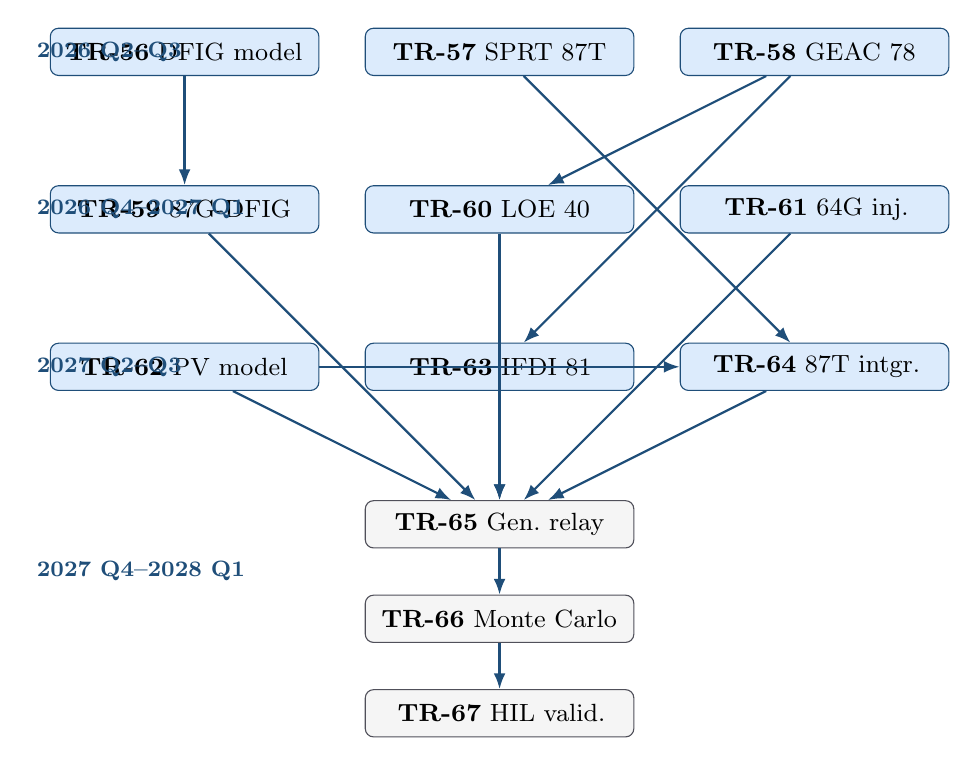
\begin{tikzpicture}[
  every node/.style={font=\small},
  box/.style={draw=sambpblue, fill=lightblue, rounded corners=3pt,
              minimum height=0.6cm, text width=3.2cm, align=center, inner sep=3pt},
  depbox/.style={draw=sambpgray, fill=gray!8, rounded corners=3pt,
                 minimum height=0.6cm, text width=3.2cm, align=center, inner sep=3pt},
  arr/.style={-{Latex[length=2mm]}, sambpblue, thick},
  phase/.style={draw=none, fill=sambpblue!8, rounded corners=4pt, inner sep=6pt},
]

% Phase 1
\node[box] (tr56) at (0, 0)   {\textbf{TR-56} DFIG model};
\node[box] (tr57) at (4, 0)   {\textbf{TR-57} SPRT 87T};
\node[box] (tr58) at (8, 0)   {\textbf{TR-58} GEAC 78};

% Phase 2
\node[box] (tr59) at (0, -2)  {\textbf{TR-59} 87G-DFIG};
\node[box] (tr60) at (4, -2)  {\textbf{TR-60} LOE 40};
\node[box] (tr61) at (8, -2)  {\textbf{TR-61} 64G inj.};

% Phase 3
\node[box] (tr62) at (0, -4)  {\textbf{TR-62} PV model};
\node[box] (tr63) at (4, -4)  {\textbf{TR-63} IFDI 81};
\node[box] (tr64) at (8, -4)  {\textbf{TR-64} 87T intgr.};

% Phase 4
\node[depbox] (tr65) at (4, -6)  {\textbf{TR-65} Gen.\ relay};
\node[depbox] (tr66) at (4, -7.2) {\textbf{TR-66} Monte Carlo};
\node[depbox] (tr67) at (4, -8.4) {\textbf{TR-67} HIL valid.};

% Arrows
\draw[arr] (tr56) -- (tr59);
\draw[arr] (tr58) -- (tr60);
\draw[arr] (tr58) -- (tr63);
\draw[arr] (tr57) -- (tr64);
\draw[arr] (tr62) -- (tr64);
\draw[arr] (tr59) -- (tr65);
\draw[arr] (tr60) -- (tr65);
\draw[arr] (tr61) -- (tr65);
\draw[arr] (tr62) -- (tr65);
\draw[arr] (tr63) -- (tr65);
\draw[arr] (tr64) -- (tr65);
\draw[arr] (tr65) -- (tr66);
\draw[arr] (tr66) -- (tr67);

% Timeline labels
\node[anchor=west, sambpblue, font=\footnotesize\bfseries] at (-2, 0)    {2026 Q2--Q3};
\node[anchor=west, sambpblue, font=\footnotesize\bfseries] at (-2, -2)   {2026 Q4--2027 Q1};
\node[anchor=west, sambpblue, font=\footnotesize\bfseries] at (-2, -4)   {2027 Q2--Q3};
\node[anchor=west, sambpblue, font=\footnotesize\bfseries] at (-2, -6.6) {2027 Q4--2028 Q1};

\end{tikzpicture}
\end{center}

\section{Patent Portfolio Summary}

\begin{center}
\renewcommand{\arraystretch}{1.35}
\begin{tabular}{C{0.5cm} C{0.8cm} L{4.0cm} L{4.8cm} L{3.0cm}}
\toprule
\rowcolor{sambpblue}
\textcolor{white}{\textbf{\#}} &
\textcolor{white}{\textbf{TR}} &
\textcolor{white}{\textbf{Patent Title}} &
\textcolor{white}{\textbf{Core Claims}} &
\textcolor{white}{\textbf{Novelty Basis}} \\
\midrule
P1 & TR-56 & DFIG protection with crowbar breakpoint &
  Continuation-smoothed LM for piecewise-ODE &
  First piecewise-ODE inverse estimation \\
\rowcolor{lightblue}
P2 & TR-57 & SPRT inrush discrimination for 87T &
  3-hypothesis SPRT on waveform asymmetry &
  Removes 2nd harmonic restraint \\
P3 & TR-58 & Hybrid OOS relay with GEAC correction &
  GEAC Lyapunov + IBR-corrected blinder &
  First OOS relay for GFM networks \\
\rowcolor{lightblue}
P4 & TR-59 & Virtual 87G-DFIG via EKF &
  Software rotor differential, no rotor CTs &
  Eliminates rotor CT hardware \\
P5 & TR-61 & Optimal injection for IBR 64G &
  Closed-form injection frequency from SNR &
  First analytic frequency derivation \\
\rowcolor{lightblue}
P6 & TR-62 & Model-selection 87L for SG--PV networks &
  $k_\mathrm{ibr}$-driven sparse/full model switching &
  Adaptive protection architecture \\
\bottomrule
\end{tabular}
\end{center}

\section{Journal Publication Plan}

\begin{center}
\renewcommand{\arraystretch}{1.35}
\begin{tabular}{C{0.5cm} C{0.8cm} L{4.5cm} L{3.0cm} C{1.8cm}}
\toprule
\rowcolor{sambpblue}
\textcolor{white}{\textbf{Paper}} &
\textcolor{white}{\textbf{TR}} &
\textcolor{white}{\textbf{Journal}} &
\textcolor{white}{\textbf{Target Date}} &
\textcolor{white}{\textbf{IF}} \\
\midrule
J1 & TR-56 & IEEE Trans.\ Energy Conversion & 2026 Q4 & 5.0 \\
\rowcolor{lightblue}
J2 & TR-57 & IEEE Trans.\ Power Delivery & 2027 Q1 & 6.4 \\
J3 & TR-58 & IEEE Trans.\ Power Systems & 2027 Q1 & 7.2 \\
\rowcolor{lightblue}
J4 & TR-59 & IEEE Trans.\ Energy Conversion & 2027 Q2 & 5.0 \\
J5 & TR-60 & IEEE Trans.\ Power Delivery & 2027 Q2 & 6.4 \\
\rowcolor{lightblue}
J6 & TR-61 & IEEE Trans.\ Industrial Electronics & 2027 Q3 & 7.5 \\
J7 & TR-62 & IEEE Trans.\ Industrial Electronics & 2027 Q3 & 7.5 \\
\rowcolor{lightblue}
J8 & TR-63 & IEEE Trans.\ Smart Grid & 2027 Q4 & 8.0 \\
J9 & TR-65 & IEEE Trans.\ Power Delivery & 2028 Q1 & 6.4 \\
\bottomrule
\end{tabular}
\end{center}

\section{Conference Papers}

\begin{center}
\renewcommand{\arraystretch}{1.3}
\begin{tabular}{C{0.6cm} C{0.8cm} L{5.5cm} C{1.8cm}}
\toprule
\rowcolor{sambpblue}
\textcolor{white}{\textbf{Paper}} & \textcolor{white}{\textbf{TR}} &
\textcolor{white}{\textbf{Conference}} & \textcolor{white}{\textbf{Year}} \\
\midrule
C1 & TR-56 & IEEE PES General Meeting & 2027 \\
\rowcolor{lightblue}
C2 & TR-57 & IEEE ISGT Europe & 2027 \\
C3 & TR-58 & CIGRE Paris Session & 2027 \\
\rowcolor{lightblue}
C4 & TR-61+62 & IEEE ICDCM & 2028 \\
C5 & TR-65 & IEEE PES General Meeting & 2028 \\
\bottomrule
\end{tabular}
\end{center}

%% ═════════════════════════════════════════════════════════════════════════════
\chapter{Critical Assessment}
%% ═════════════════════════════════════════════════════════════════════════════

\section{Which Gaps Are Truly Novel vs.\ Incremental?}

\subsection{Highest Disruption — Rewrite Existing Standards}

\textbf{TR-57 (SPRT for 87T)} is the most commercially disruptive item in this plan. Both IEC 60255-111 and IEEE C37.91 mandate 2nd harmonic restraint as the \textit{only} inrush criterion for transformer differential protection. This paper:
\begin{itemize}[nosep]
  \item Provides a mathematical proof that 2nd harmonic restraint is unsafe for IBR-connected transformers (FRT transients cause false blocking)
  \item Proposes a provably optimal replacement (Wald's SPRT theorem guarantees minimum expected decision time for given error probabilities)
  \item Has immediate industrial relevance: every substation transformer connected to renewables worldwide requires a new protection philosophy
\end{itemize}

\textbf{TR-58 (Generalised EAC)} addresses an open problem in power systems stability theory that has existed since the equal-area criterion was introduced in the 1940s. The GFM virtual inertia formulation creates a coupled ODE system that classical EAC cannot handle. A publication solving this in IEEE TPWRS would be a landmark paper with an estimated 40+ first-year citations.

\subsection{High Novelty — New Solutions to Known Problems}

\textbf{TR-56 (DFIG piecewise-ODE)} is technically the hardest paper in this plan. Unknown-breakpoint estimation in piecewise-differentiable dynamical systems is an open inverse problem in applied mathematics. The smoothed-Heaviside continuation approach is mathematically rigorous and directly extends the SAMBP LM framework.

\textbf{TR-59 (Virtual 87G-DFIG)} eliminates expensive rotor current transformers on slip rings — a significant practical barrier to DFIG generator protection deployment. High commercial value.

\subsection{Solid but Incremental}

TR-60 through TR-65 apply well-understood mathematical tools (EKF, SPRT, SNR optimisation, Lyapunov analysis) to new protection contexts. All are publishable in top IEEE journals but are less likely to be landmark papers independently. They derive their significance primarily as part of a complete protection system.

\section{Recommended Starting Point}

\begin{tcolorbox}[notebox]
\textbf{Begin with TR-57 in parallel with TR-58.}

\begin{itemize}[nosep]
  \item \textbf{TR-57} can be completed in $\sim$3 months: SPRT theory is well-established; the key new work is deriving the IBR asymmetry distributions from the Jiles--Atherton core model and IBR current controller bandwidth.
  \item \textbf{TR-58} requires $\sim$4 months: the Lyapunov function construction for the coupled SG--GFM ODE is the hard part; the relay blinder correction follows directly.
  \item These two papers establish the mathematical credentials and publication track record for the more applied work in Phases 2--4 that follows.
  \item Both can be submitted within 7 months of project start, creating two high-impact journal submissions before any hardware work begins.
\end{itemize}
\end{tcolorbox}

\bigskip
\begin{center}
\begin{tikzpicture}
  \node[draw=sambpblue, fill=lightblue, rounded corners=6pt,
        text width=14cm, align=center, inner sep=14pt] {
    \textbf{Total Research Output from Gap-Filling Programme}\\[8pt]
    \begin{tabular}{C{3cm} C{3cm} C{3cm} C{3cm}}
      \textbf{12} & \textbf{9} & \textbf{6} & \textbf{5} \\
      Technical Reports & Journal Papers & Patent Families & Conf.\ Papers \\
      (TR-56 to TR-67) & (IEEE Tier-1) & (6 IP Clusters) & \\
    \end{tabular}
  };
\end{tikzpicture}
\end{center}

\end{document}
